\documentclass[titlepage,12pt,a4paper]{article}
\usepackage[T1]{fontenc}
\usepackage[utf8]{inputenc}
\usepackage[brazil]{babel}
\usepackage{indentfirst}
\usepackage{graphicx}
\usepackage[datesep=/,style=ddmmyyyy]{datetime2}
\usepackage[hidelinks]{hyperref}
\usepackage[section]{placeins}
\usepackage{float}
\floatstyle{boxed}
\restylefloat{figure}
\restylefloat{table}

\begin{document}

  \begin{titlepage}
    \centering
      {\scshape\LARGE Universidade Federal do Rio Grande Do Sul \par}
      {\scshape\Large Instituto de Informática \par}
      {\large Departamento de Informática Aplicada \par}
      {\large INF01124 - Classificação e Pesquisa de Dados - Turma B \par}
      \vfill
      {\LARGE Exercício 1 \par}
      \vfill
      {\raggedright\large Autor: Felipe de Almeida Graeff \par}
      {\raggedright\large Cartão: 00261606 \par}
      \vspace{5cm}
      \today
  \end{titlepage}

  \section{INTRODUÇÃO}

    Modelos matemáticos de computação como a máquina de Turing prevêem recursos
    de tempo e memória infinitos, porém a realidade impõe limitações para esses
    recursos. Gács e Lovász(1999)\cite{gacslovasz99} explicam que, limitando-se
    os recursos disponíveis para a computação de um problema, a quantidade de
    problemas que podemos resolver também é limitada. Por esse motivo é
    de extrema importância o estudo e o entendimento de conceitos da área da
    complexidade de algoritmos, para que possamos criar algoritmos mais
    eficientes e que necessitem menos recursos, tanto de tempo como de memória.

  \section{OBJETIVOS}

    Em um primeiro momento, observar e classificar diferentes comportamentos de
    funções para entender seus impactos no que se refere à complexidade de
    algoritmos. Após isso gerar dados para comparação de 2 algoritmos de ordenamento
    a partir de três implementações distintas, sendo uma de Bubble Sort e duas
    de Shell Sort.

  \section{IMPLEMENTAÇÃO E PROGRAMAS UTILIZADOS}

    Para a coleta dos dados foram utilizadas implementações do Shell Sort e do
    Bubble Sort na linguagem de programação C$++$. A compilação foi feita com o
    compilador g$++$ utilizando a flag de otimização ``-O2''.Para todos os testes
    foi utilizado o mesmo array, gerado aleatoriamente com a seed 1.

    Os gráficos e tabelas apresentadas na seção~\ref{sec:anexos} foram criados a
    partir dos dados de saída do programa principal. Os gráficos foram criados
    pela ferramenta gnuplot e as tabelas foram feitas com \LaTeX.

    Para a comparação das funções apresentadas na subseção~\ref{subsec:complex}
    também foi utilizada a ferramenta gnuplot.

    Todos os códigos fonte podem ser conferidos no repositório disponível através
    do link \textless\url{http://github.com/Fxlipe115/CPD_Sorting}\textgreater(acesso em: \today).

  \section{RESULTADOS}

    \subsection{COMPLEXIDADE DE FUNÇÕES}
      \label{subsec:complex}

      A partir da análise dos gráficos das funções requisitadas foi criada a
      tabela~\ref{tab:complex} que contém as funções ordenadas de acordo com suas
      ordens de complexidades, da mais baixa para a mais alta. A tabela pode ser
      conferida na seção~\ref{sec:anexos} deste relatório.

    \subsection{SHELL SHORT}

      Nesta subseção serão comparados os dados gerados pela execução de duas
      implementações do algoritmo Shell Sort, uma utilizando a sequência
      $[1,2,4,8,16,32,64,\ldots]$ (referida neste relatório como implementação $1$)
      e a outra utilizando a sequência $[1,4,13,40,121,\ldots]$ (implementação $2$)
      para o cálculo do número de segmentos em cada iteração, para entradas de
      $10,000$ e de $100,000$ elementos.

      \subsubsection{Entrada com $10,000$ elementos}

        Para a implementação $1$ o algoritmo realizou $14$ iterações fazendo um
        total de $409,280$ trocas. A implementação $2$ fez $9$ iterações realizando
        $131,250$ trocas.

        A relação entre as trocas feitas em cada iteração com o número de segmentos
        gerados pode ser visualizada nas tabelas \ref{tab:10000seq1} e \ref{tab:10000seq2}.

      \subsubsection{Entrada com $100,000$ elementos}

        Com uma entrada de $100,000$ elementos a implementação $1$ fez $17$ iterações
        e um total de $20,750,386$ trocas. A implementação $2$ fez $11$ iterações
        e $2,835,159$ trocas.

        A quantidade de segmentos e o número de trocas feitas em cada iteração
        pode ser visto nas tabelas \ref{tab:100000seq1} e \ref{tab:100000seq2}.

      \subsubsection{Comparação temporal}

        A implementação $1$ ordenou $10,000$ itens em $0.002$ segundos e $100,000$
        itens em $0.075$ segundos. A implementação $2$ ordenou $10,000$ elementos
        em $0.002$ segundos e $100,000$ elementos em $0.022$ segundos.

        O gráfico da figura~\ref{fig:grafs1s2} mostra o comportamento relativo ao tempo das
        duas implementações para entradas que vão de $10,000$ até $1,000,000$ elementos.

    \subsection{BUBBLE SORT}

      Para o teste com o Bubble Sort foi utilizado o mesmo array de $10,000$ elementos
      usado nos testes com o Shell Sort.

      O Bubble Sort levou $0.2$ segundos para ordenar os $10,000$ elementos, fazendo
      $25,341,218$ trocas no processo.

      O gráfico da figura~\ref{fig:grafs1s2b} mostra o comportamento do Bubble Sort, em
      relação às duas implementações de Shell Sort vistas anteriormente, para um
      intervalo de tempo de até 1 minuto.

  \section{CONCLUSÃO}

    Analizando os gráficos e comparando os dados, ficou claro que o algoritmo
    Shell Sort com a implementação $1$ foi o mais eficiente entre os $3$
    implementados. A implementação 2, embora tenha tido o mesmo comportamento e
    tenha a mesma complexidade, teve um pior desempenho por fazer a segmentação
    da entrada de forma não tão ótima quanto a implementação 1. Isso ocasionou
    um maior número de iterações em comparação com aquela e, consequentemente,
    um tempo maior de processamento, para entradas de mesmo tamanho.

    O Bubble Sort obteve um desempenho consideravelmente inferior ao de ambas
    as implementações de Shell Sort. Isso ocorreu devido ao comportamento polinomial
    do algoritmo que pôde ser observado no gráfico da figura~\ref{fig:grafs1s2b}.

  \section{ANEXOS}
    \label{sec:anexos}

    \begin{table}[h]
      \caption{Complexidades \label{tab:complex}}
      \begin{center}
        \begin{tabular}{ l }
          $ln(ln(n)$ \\
          $\sqrt{lg(n)}$ \\
          $lg(n)$ \\
          $lg(n)^2$ \\
          $\sqrt{n}$ \\
          $n$ \\
          $n^2$ \\
          $n^3$ \\
          $e^n$ \\
          $n!$
        \end{tabular}
      \end{center}
    \end{table}

    \begin{table}[h]
      \caption{Implementação $1$ de Shell Sort com $10,000$ elementos \label{tab:10000seq1}}
      \begin{center}
        \begin{tabular}{ r | r | r }
          Iteração & Segmentos & Trocas \\
          \hline \\
          1 & 8192 & 918 \\
          2 & 4096 & 2429 \\
          3 & 2048 & 3258 \\
          4 & 1024 & 4840 \\
          5 & 512 & 6813 \\
          6 & 256 & 9497 \\
          7 & 128 & 13744 \\
          8 & 64 & 18485 \\
          9 & 32 & 25168 \\
          10 & 16 & 33866 \\
          11 & 8 & 56893 \\
          12 & 4 & 103897 \\
          13 & 2 & 56453 \\
          14 & 1 & 154019
        \end{tabular}
      \end{center}
    \end{table}

    \begin{table}[h]
      \caption{Implementação $2$ de Shell Sort com $10,000$ elementos \label{tab:10000seq2}}
      \begin{center}
        \begin{tabular}{ r | r | r }
          Iteração & Segmentos & Trocas \\
          \hline \\
          1 & 9841 & 94 \\
          2 & 3280 & 5052 \\
          3 & 1093 & 9537 \\
          4 & 364 & 14233 \\
          5 & 121 & 20397 \\
          6 & 40 & 25028 \\
          7 & 13 & 39041 \\
          8 & 4 & 31930 \\
          9 & 1 & 15938
        \end{tabular}
      \end{center}
    \end{table}

    \begin{table}[h]
      \caption{Implementação $1$ de Shell Sort com $100,000$ elementos \label{tab:100000seq1}}
      \begin{center}
        \begin{tabular}{ r | r | r }
          Iteração & Segmentos & Trocas \\
          \hline \\
          1 & 65536 & 17236 \\
          2 & 32768 & 17562 \\
          3 & 16384 & 38259 \\
          4 & 8192 & 55709 \\
          5 & 4096 & 78350 \\
          6 & 2048 & 107211 \\
          7 & 1024 & 152645 \\
          8 & 512 & 220229 \\
          9 & 256 & 310765 \\
          10 & 128 & 425564 \\
          11 & 64 & 657542 \\
          12 & 32 & 860052 \\
          13 & 16 & 1271892 \\
          14 & 8 & 1666816 \\
          15 & 4 & 2554169 \\
          16 & 2 & 4126619 \\
          17 & 1 & 8189766
        \end{tabular}
      \end{center}
    \end{table}

    \begin{table}[h]
      \caption{Implementação $2$ de Shell Sort com $100,000$ elementos \label{tab:100000seq2}}
      \begin{center}
        \begin{tabular}{ r | r | r }
          Iteração & Segmentos & Trocas \\
          \hline \\
          1 & 88573 & 5674 \\
          2 & 29524 & 50157 \\
          3 & 9841 & 93910 \\
          4 & 3280 & 147248 \\
          5 & 1093 & 201697 \\
          6 & 364 & 272576 \\
          7 & 121 & 369239 \\
          8 & 40 & 541906 \\
          9 & 13 & 669922 \\
          10 & 4 & 356081 \\
          11 & 1 & 126749
        \end{tabular}
      \end{center}
    \end{table}

    \begin{figure}[h]
      \caption{Gráfico comparativo Shell Sort \label{fig:grafs1s2}}
      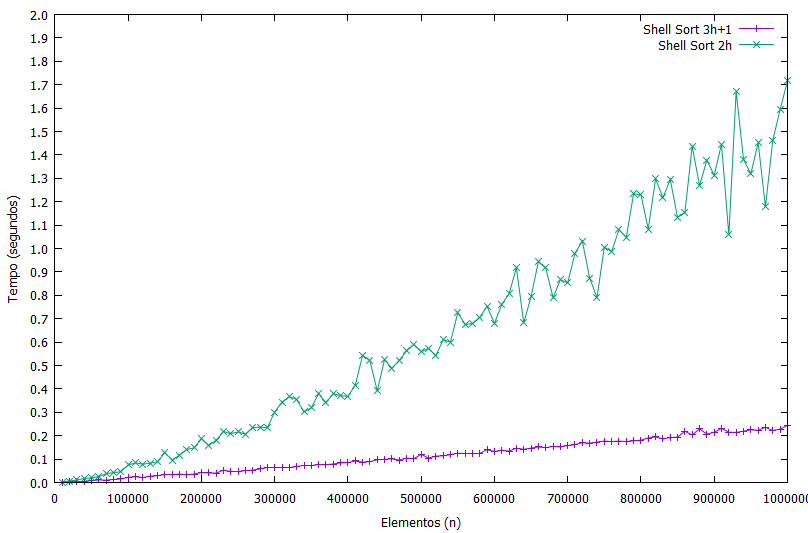
\includegraphics[width=\textwidth]{../data/plots/plot_S1S2_O2.png}
    \end{figure}

    \begin{figure}[h]
      \caption{Gráfico comparativo com Bubble Sort \label{fig:grafs1s2b}}
      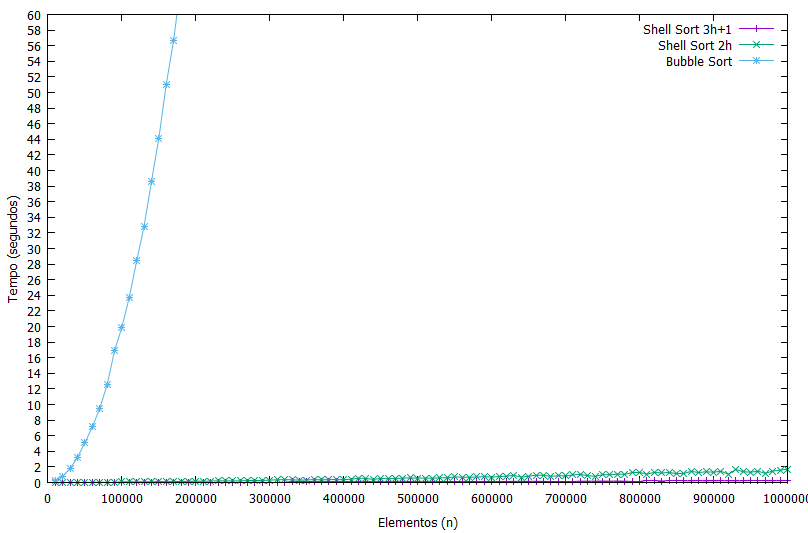
\includegraphics[width=\textwidth]{../data/plots/plot_S1S2B_O2.png}
    \end{figure}

  \FloatBarrier

  \begin{thebibliography}{9}

    \bibitem{gacslovasz99}
      Gács, P.;
      Lovász, L.
      (1999).
      \emph{Complexity of Algorithms}.
      Lecture Notes,
      Yale University.
      Disponível em \textless\url{http://www.esi2.us.es/~mbilbao/pdffiles/complex.pdf}\textgreater%
      (Acesso em: \today).

  \end{thebibliography}

\end{document}
